\section{The Real and Complex Number Systems}
\subsection{The Naturals, Integers, and Rationals}
We begin by a review of number systems which are already familiar.

\begin{ndef}{The Natural Numbers}
    The \textbf{Naturals}, denoted by $\NN$, is the set $\set{1, 2, 3, \ldots}$.
\end{ndef}

\noindent For $x, y, \in \NN$, we have that $x + y \in \NN$ and $xy \in \NN$, so the naturals are closed under addition and multiplication. However, we note that it is not closed under subtraction; take for example $2 - 4 = -2 \notin \NN$.

\begin{ndef}{The Integers}
    The \textbf{Integers}, denoted by $\ZZ$, is the set $\set{\ldots, -3, -2, -1, 0, 1, 2, 3, \ldots}$.
\end{ndef}

\noindent The integers are closed under addition, multiplication, and subtraction. However, it is not closed under division; for example, $1/2 \notin \ZZ$. 

\begin{ndef}{The Rationals (informal)}
    The \textbf{Rationals}, denoted by $\QQ$, can be defined as $\set{\frac{m}{n}: m \in \ZZ, n \in \NN}$, where $\frac{m_1}{n_1}$ and $\frac{m_2}{n_2}$ are identified if $m_1n_2 = m_2n_1$.
\end{ndef}

\noindent We note that unlike the naturals/integers, the rationals do not have as obvious of a denumeration. This above is a good definition if we already have the same rigorous idea of what a rational number is in our mind; i.e. it works because we have a shared preconceived understanding of a rational number.

If this is not the case, it may help to define the rational numbers more rigorously/formally (even if the definition may be slightly harder to parse). As a second attempt at a definition, we can say that $\QQ$ is the set of ordered pairs $\set{(m, n): m \in \ZZ, n \in \NN}$. However, this is not quite enough as we need a notion of equivalence between two rational numbers (e.g. $(1, 2) = (2, 4)$). Hence, a complete and rigorous definition would be:

\begin{ndef}{The Rationals (formal)}
    The \textbf{Rationals}, denoted by $\QQ$, is the set $\set{(m, n): m \in \ZZ, n \in \NN}/\sim$ where $(m_1, n_1) \sim (m_2, n_2)$ if $m_1n_2 = m_2n_1$.
\end{ndef}
\noindent Under the formal definition, the rationals are a set of equivalence classes of ordered pairs, under the equivalence relation $\sim$. We note that the rationals are closed under addition, subtraction, multiplication, and division.

This formal definition might be slightly harder to parse, so it might be useful to consider an example with a similar flavour. Consider the set $X = \set{m \in \ZZ}/\sim$ such that $m_1 \sim m_2$ if $m_1 - m_2$ is divisible by 12. This is "clock arithmetic", with equivalence classes $[0], [1], [2], \ldots$ for each hour on an analog clock. A fun side note: If instead of 12 we picked a prime number, we would get a field (we will discuss what this is in a later lecture)!

Note that under this definition, $(1, 2)$ and $(2, 4)$ are different representations of the same rational number. With this definition, we would define addition such that $(m_1, n_1) + (m_2, n_2) = (m_1n_2 + m_2n_1, n_1n_2)$. Note that $(2m_1, 2n_2) + (m_2, n_2) = (2m_1n_2 + 2m_2n_1, 2n_1n_2)$ and we can identify $(m_1n_2 + m_2n_1, n_1n_2)$ with $(2m_1n_2 + 2m_2n_1, 2n_1n_2)$. If we choose different representations when we do addition, we might get a different representation in our result, but it will represent the same rational number regardless of the choice of representations we originally chose to do the addition. 

A natural question then becomes if the rationals are sufficient for doing all of real analysis. Certainly, it seems as we have a number system that is closed under all our basic arithmetic operations; but is this enough? For example, are we able to take limits just using the rationals? The answer turns out to be no (they are insufficient!) and the following example will serve as one illustration of this fact. 

\begin{example}{Incompleteness of the Rationals}{1.1a}
    There exists no $p \in \QQ$ such that $p^2 = 2$.
\end{example}
\noindent We proceed via proof by contradiction. Recall in that these types of proof, we start with a certain wrong assumption, follow a correct/true line of reasoning, reach an eventual absurdity, and therefore conclude that the original assumption was mistaken. 
\begin{nproof}
    Let us then suppose for the contradiction that there exists $p = \frac{m}{n}$ with $p^2 = 2$. We then have that not both $m, n$ are even, and hence at least one is odd. Then, we have that $2 = p^2 = \frac{m^2}{n^2}$ and hence $m^2 = 2n^2$, so $m^2$ is even, implying $m$ is even. So, let us write $m = 2k$ for $k \in \ZZ$. Then, $(2k)^2 = 4k^2 = 2n^2$, and hence $2k^2 = n^2$. Therefore, $n^2$ is even and hence $n$ is even. $m$ and $n$ are therefore both even, a contradiction. We conclude that no such $p$ exists. \qed
\end{nproof}
\noindent Why can we conclude that not both $m, n$ are even in the above proof? This is the case as if $m, n$ we both even, then we could write $m = 2m'$, $n = 2n'$ for some $m', n'$, and then $p = \frac{m}{n} = \frac{2m'}{2n'} = \frac{m'}{n'}$ which we can continue until either the numerator or denominator is odd. A natural question to consider is how to prove that this process of reducing fractions will eventually conclude. The resolution is to invoke the fundamental theorem of arithmetic, and write $m, n$ in terms of their unique prime factorization. We are then able to cancel out factors of 2 from the numerator/denominator until at least one is odd.

We note that this example leads us to conclude that the rationals have certain "holes" in them. This is concerning, as there are sequences of rational numbers that tend to $\sqrt{2}$. Conversely, its not as concerning that there is no rational number $x$ such that $x^2 = -1$, as there is no such sequence of rational numbers that is "close to" $i$ (note that both $\sqrt{2}$ and $i$ have not yet been defined, but this will come shortly).

\setcounter{rudin}{0}

\begin{example}{Incompleteness of the Rationals}{1.1b}
    Let $A = \set{p \in \QQ: p > 0, p^2 < 2}$, and $B = \set{p \in \QQ: p > 0, p^2 > 2}$. Then, $\forall p \in A, \exists q \in A$ such that $p < q$, and $\forall p \in B, \exists q \in B$ such that $q < p$. 
\end{example}
\begin{figure}[htbp]
    \centering
    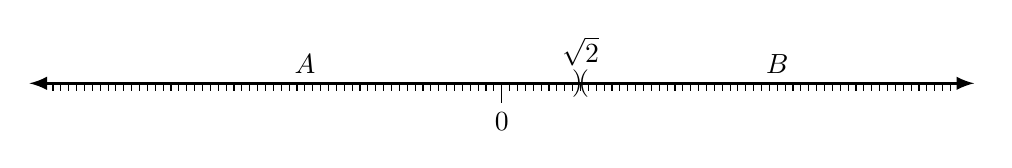
\begin{tikzpicture}
        \draw[latex-latex, very thick] (-6, 0) -- (6,0) node[anchor=south] {$\QQ$};
        \draw[] (0, 0) -- (0, -0.25) node[anchor=north] {0};
        \foreach \i in {-5.7,-5.6,...,5.7}{ 
        \draw[] (\i,0) -- (\i,-0.1);
        }
        \draw[] (1,0.1) node[anchor=south] {$\sqrt{2}$};
        \draw[] (0.96,0) node[] {$)$};
        \draw[] (1.04,0) node[] {$($};
        \draw[] (-2.5, 0) node[anchor=south] {$A$};
        \draw[] (3.5, 0) node[anchor=south] {$B$};
    \end{tikzpicture}
    \caption{Visualization of sets $A$ and $B$. We note that $\sqrt{2}$ has not been defined in our formalism yet, but from our prior mathematical intuition it would be what goes in the "hole" of the rationals.}
    \label{fig1}
\end{figure}

\noindent For the proof of this statement, we consider playing a 2 person game. One person is $\forall$, one person is $\exists$, and we consider if one person has a winning strategy. $\forall$ goes first, and then $\exists$ goes next, having seen the choice that $\forall$ has made. Then, we check if indeed $p < q$. If $p < q$, then $\exists$ wins. If $p \not< q$, then $\forall$ wins. 

\begin{nproof}
    Let $p \in A$. Then, let $q = \frac{2p + 2}{2 + p}$. Since $p \in \QQ$, it follows that $2p + 2 \in \QQ$ and $2 + p \in \QQ$ so $q \in \QQ$. Furthermore, we have that $2p + 2 > 0$ and $2 + p > 0$, so $q > 0$. We also have that:
    \[q^2 = \frac{(2p+2)^2}{(2+p)^2} = 2 + \frac{2(p^2 - 2)}{(p+2)^2} < 2\]
    Where the inequality follows from the fact that $p^2 < 2$ and hence $(p^2 - 2) < 0$. It therefore follows that $q \in A$. Finally, we have that:
    \[q = p + \frac{2-p^2}{2+p} > p\]
    so $q > p$, completing the proof of the first part of the claim. The second part is left as an exercise (we note that the same $q$ can be used). \qed
\end{nproof}

\noindent The number $q = \frac{2p+ 2}{2 + p}$ seems to be pulled out of a hat, but actually comes from a fairly geometric picture (the secant method of approximating roots). Discussion on this topic can be found here: \\ \texttt{https://math.stackexchange.com/questions/141774/choice-of-q-in-baby-rudins-example-1-1}.

\subsection{Ordered Sets}
Over the next couple sections, we will be discussing certain properties of sets that will give us a better understanding of the real numbers, and allow us to construct them.

\setcounter{rudin}{4}

\begin{definition}{Order}{1.5}
    An \textbf{order} $<$ on a set $S$ is a relation with the following properties:
    \begin{enumerate}[(i)]
        \item For every pair $x, y \in S$, exactly one of $x < y$, $x = y$, or $y < x$ is true. 
        \item For $x, y, z \in S$, if $x < y$ and $y < z$, then $x < z$. 
    \end{enumerate}
    A point on notation; We note that $x > y$ means $y < x$, and $x \leq y$ means $x < y$ or $x = y$. 
\end{definition}

\begin{definition}{Ordered Sets}{1.6}
    An ordered set is a pair $(S, <)$. We may write just $S$ if the order can be inferred by the context.
\end{definition}
\noindent A familiar (and useful) set of examples is $S = \NN$ or $S = \ZZ$ or $S = \QQ$. For these three sets, we have that $x < y$ if $y-x$ is positive. For another example, consider the set $S$ of english words; then the order $<$ can be the dictionary/lexographic order. 

\begin{definition}{Upper \& Lower Bounds}{1.7}
    Let $S$ be an ordered set and $E \subset S$ (note that here, $E \subset S$ is a non-strict subset, and $E \subsetneq S$ is a strict subset). $E$ is \textbf{bounded above} if there exists an element $\beta \in S$ such that $\forall x \in E$, $x \leq \beta$. Any such $\beta$ is an \textbf{upper bound} of $E$. Similarly, we say that $E$ is \textbf{bounded below} if there exists an element $\alpha \in S$ such that $\forall x \in E$, $\alpha \leq x$. In this case, $\alpha$ is a \textbf{lower bound} of $E$.
\end{definition}
\noindent As an example, one can take $S = \QQ$, $E = A = \set{p \in \QQ: p > 0, p^2 > 2}$ (as in Example \ref{exam:1.1b}). Here, $E$ is bounded above, with $\beta = 2$ as one possible upper bound. to see this is the case, consider that if $p \in E$:
\[2 - p = \frac{4 - p^2}{2+p} > \frac{4-2}{2+p} > 0\]
\noindent However, if we take $S = A$, $E = A$, then $E$ is not bounded above as we saw in the example. There is no upper bound of $A$ in $A$. In general, this example reveals the subtle point that "the upper bound of a set" is ill-defined; we need to specify $E \subset S$. 

\subsection{The Least Upper Bound Property}
\begin{definition}{Least Upper Bound \& Greatest Lower Bound}{1.8}
    Let $S$ be an ordered set, and let $E \subset S$ with $E$ bounded above. If $\exists \alpha \in S$ such that:
    \begin{enumerate}[(i)]
        \item $\alpha$ is an upper bound for $E$
        \item If $\gamma < \alpha$, then $\gamma$ is not an upper bound for $E$
    \end{enumerate} 
    The $\alpha$ is the \textbf{least upper bound}, or \textbf{supermum} of $E$. This can be denoted as $\alpha = \sup(E)$. Analogously, the \textbf{greatest lower bound}, or \textbf{infimum} of E (denoted $\alpha = \inf(E)$) is an element $\alpha \in S$ (if it exists) such that:
    \begin{enumerate}[(i)]
        \item $\alpha$ is a lower bound for $E$
        \item If $\gamma > \alpha$, then $\gamma$ is not an upper bound of $E$. 
    \end{enumerate}
\end{definition}

\begin{ntheorem}{Uniqueness of supremum/infimum}
    If the supremum/infimum of $E \subset S$ exist, they are unique.
\end{ntheorem}
\begin{nproof}
        Let $E \subset S$. Suppose that there exist $\alpha_1, \alpha_2$ such that $\alpha_1 = \sup(E)$ and $\alpha_2 = \sup(E)$. If $\alpha_1 < \alpha_2$, as $\alpha_1$ is an upper bound of $E$, this contradicts the fact that $\alpha_2$ is the least upper bound of $E$. We reach an identical contradiction if $\alpha_2 < \alpha_1$. Therefore we conclude that $\alpha_1 = \alpha_2$ and the supremum of $E$ is unique (if it exists). The proof for the infimum is analogous. \qed
\end{nproof}

\begin{ntheorem}{Equivalence of maximum and supremum}
    If $E \subset S$ has a maximum element $\alpha$ (that is, an element such that $x < \alpha$ for all $x \in E$) then $\alpha = \sup(E)$. Similarly, if $E$ has a minimum element $\alpha$, then $\alpha = \inf(E)$. The proof is left as an exercise. 
\end{ntheorem}

\begin{comment}
\begin{nproof}
    Let $E \subset S$ and $\alpha = \max(E)$. By definition $\alpha$ is an upper bound of $E$, and if $x < \alpha$ for some $x \in E$ then $x$ is not an upper bound of $E$ as it is not greater than $\alpha \in E$. The claim follows (with an identical proof for the minimum). \qed
\end{nproof}
\end{comment}

\begin{example}{}{1.9}
    \begin{enumerate}
        \item Consider again the sets $A, B \subset \QQ$ from example \ref{exam:1.1b}. $A$ is bounded above by any element in $B$, and the upper bounds of $A$ are exactly the elements of $B$. Since $B$ has no smallest member, $A$ does not have a least upper bound in $\QQ$.
        \item Let $E_1, E_2 \subset \QQ$ such that $E_1 = \set{r: \QQ, r < 0}$ and $E_2 = \set{r: \QQ, r \leq 0}$. Then $\sup(E_1) = \sup(E_2) = 0$. Note that this example shows that the supremum can either be contained or not contained in the set; $0 \notin E_1$ but $0 \in E_2$. 
        \item Let $E \subset \QQ$ such that $E = \set{\frac{1}{n}: n \in \NN}$. Then $\sup(E) = 1$ and $\inf(E) = 0$. This is proven below. 
    \end{enumerate}
\end{example}
\begin{nproof}
    $\sup(E) = 1$ immediately follows from the equivalence of the maximum and supremum as proven above. To see that $\inf(E) = 0$, first note that $0$ is a lower bound for $E$ as all of the elements of $E$ are positive. To see that it is the lower bound, take any $x > 0$. Then, we have that for any $n > \frac{1}{x}$, $\frac{1}{n} < x$ and hence $x$ is not an upper bound of $E$. This proves the claim. \qed
\end{nproof}

\begin{definition}{The LUB/GUB Property}{1.10}
    An ordered set $S$ has the \textbf{least upper bound property} if for every $E \subset S$, if $E \neq \emptyset$ and $E$ is bounded above, then $E$ has a least upper bound (that is, $\sup(E)$ exists in $S$). Similarly, an ordered set $S$ has the \textbf{greatest lower bound property} if for every $E \subset S$, if $E \neq \emptyset$ and $E$ is bounded below, then $E$ has a greatest lower bound.
\end{definition}
\noindent We will show in the next theorem that these properties are actually equivalent; before then, we briefly consider two examples.
\begin{nexample}{$\ZZ$ and $\QQ$}
    $\ZZ$ has the least upper bound property, while $\QQ$ does not. 
\end{nexample}
\begin{nproof}
    For the first claim, consider any nonempty $E \subset \ZZ$ that is bounded above. Choose any $x \in E$. Since $\ZZ$ is bounded above, there exist finitely many elements that are greater than $x$. Take the maximum of these finitely many elements. This maximum is also the maximum of $E$, so it is the supremum of $E$. Therefore $\ZZ$ has the LUB property as claimed.
    
    The second claim immediately follows from Example \ref{exam:1.9}(a). \qed
\end{nproof}

\begin{theorem}{Equivalence of LUB/GUB properties}{1.11}
    Let $S$ be an ordered set. Then $S$ has the LUB property if and only if it has the GUB property. 
\end{theorem}
\begin{nproof}
    $\boxed{\implies}$ Let $S$ be an ordered set with the LUB property. Let $E \subset S$ with $E \neq \emptyset$, with $E$ bounded below. Let $L = \set{x \in S: x\text{ is a lower bound of $E$.}}$. $L \neq \emptyset$ as $E$ is bounded below (and hence has at least one lower bound). If $y \in E$, then $y$ is an upper bound for $L$. Since $E$ is nonempty, $L$ is therefore bounded above. Since $S$ has the LUB property, then $\sup(L)$ must exist. Let us call this $\alpha$. Then, $\alpha \leq x\ \forall x \in E$ (as if $\gamma < \alpha$, then $\gamma$ is not an upper bound of $L$ and hence $\gamma \neq E$). Hence, $\alpha$ is a lower bound for $E$ and hence $\alpha \in L$. Since $\alpha = \sup(L)$ and $\alpha$ is an upper bound for $L$, we have that $\alpha \geq \gamma\ \forall \gamma \in L$. Thus, $\alpha = \inf(E)$. 

    $\boxed{\impliedby}$ Left as an exercise. \qed
\end{nproof}

\subsection{Fields and Ordered Fields}
\begin{definition}{Fields}{1.12}
    A field $F$ is a set with two binary operations, $+$ and $\cdot$ (addition and multiplication) such that the following axioms are satisfied:
    \begin{enumerate}[start=1, label={(A\arabic*):}]
    \item If $x, y \in F$, then $x + y \in F$. (Closure under addition)
    \item $x + y = y + x$ for all $x, y \in F$. (Commutativity of addition)
    \item $(x+y) + z = x + (y + z)$ for all $x, y, z \in F$. (Associativity of addition)
    \item $\exists 0 \in F$ such that $\forall x \in F$, $0 + x = x$. (Additive identity)
    \item $\forall x \in F$, $\exists y$ such that $x + y = 0$. We can denote $y = -x$. (Additive inverse)
    \end{enumerate}
    \begin{enumerate}[start=1, label={(M\arabic*):}]
        \item If $x, y \in F$, then $x\cdot y\in F$. (Closure under multiplication)
        \item $x \cdot y = y \cdot x$ for all $x, y \in F$.
        \item $(x\cdot y)\cdot z = x \cdot (y \cdot z)$ for all $x, y, z \in F$. (Associativity under multiplication)
        \item $\exists 1 \in F$ such that $1 \neq 0$ and $\forall x \in F$, $1 \cdot x = x$. (Multiplicative identity)
        \item $\forall x \in F$, exists $y \in F$ such that $x \cdot y = 1$. We can denote $y = \frac{1}{x}$. (Multiplicative inverse)
    \end{enumerate}
    (D): $x \cdot (y + z) = x \cdot y + x \cdot z$, $\forall x, y, z \in F$. (Distributive law)
\end{definition}
\noindent Note that A3/M3 show that $x + y + z$ and $x\cdot y\cdot z$ are well defined in a mathematical sense; however, associativity may not hold for computers that do math with finite precision! 
\begin{ntheorem}{Uniqueness of Identities and Inverses}
    The additive/multiplicative identities given by (A4)/(M4) and the additive/multiplicative inverses given by (A5)/(M5) are unique. 
\end{ntheorem}
\begin{nproof}
    Let $F$ be an ordered field. Suppose that there exist $0_1, 0_2 \in F$ such that $0_1 + x= x$ and $0_2 + x = x$ for all $x \in F$. We then have that:
    \begin{align*}
        0_1 + 0_2 &= 0_1 + 0_2
        \\ 0_1 + 0_2 &= 0_2 + 0_1 & \text{(A2)}
        \\ 0_2 &= 0_1 & \text{(Property of additive identity)}
    \end{align*}
    Which shows that the additive identity is unique. The remaining proofs are left as an exercise. \qed
\end{nproof}
\noindent Some easy (and familiar) consequences of the field axioms can be found in Rudin 1.14-1.16. Instead of repeating those here, we will discuss some examples. 

The rationals form a field (under the usual notions of addition/multiplication), but the integers do not, as there are no multiplicative inverses (e.g. there exists no integer $x \in \ZZ$ such that $2\cdot x = 1$). The simplest example of a field is $F = \set{0, 1}$, with the relations:
\begin{align*}
    0 + 0 = 0\quad 0\cdot0 = 1
    \\ 0 + 1 = 0 \quad 0 \cdot 1 = 0
    \\ 1 + 1 = 0 \quad 1 \cdot 1 = 1
\end{align*}
This field is often called $\mathbb{F}_2$ or $F_2$, and is useful in computer science (where bits can take on two states, 0 or 1). As a slight tangent, a byte (8 bits) can be considered an element of an 8-dimensional vector space over the field $\mathbb{F}_2$, where $+$ would be the XOR operator and $\cdot$ would be the AND operation. 

A generalization of the above example is $\mathbb{F}_p$ or $F_p$, for a prime number $p$. This field would consist of the elements $0, 1, \ldots, p-1$. The addition and multiplication are carried out mod $p$. An interesting result is that in general, finite fields must have cardinality of some prime power. 

Note that a field cannot have a single element; the field axioms (A4) and (M4) require the existence of distinct additive and multiplicative identities, which a singleton set cannot satisfy. 

Although algebra is not the focus of this course, it may be interesting to briefly think about sets with less structure than a field. We start by considering a group. 

\begin{ndef}{Groups}
A \textbf{group} $G$ is a set with a binary operation $(a,b) \mapsto a\cdot b$ such that the following axioms are satisfied:
\begin{enumerate}[start=1, label={(M\arabic*):}]
    \item If $a, b \in G$, then $a\cdot b \in G$ (Closure)
    \stepcounter{enumi}
    \item For $a, b, c \in G$, $(a\cdot b)\cdot c = a\cdot(b\cdot c)$ (Associativity)
    \item There exists $1 \in G$ such that $\forall x \in G$, $1 \cdot x = x$. (Identity)
    \item $\forall x \in G$, there exists $y \in G$ such that $x \cdot y = 1$. (Inverse) 
\end{enumerate}
\end{ndef}
\noindent We note that $\ZZ$ is a group under addition, but not under multiplication (due to lack of multiplicative inverses). We can also consider the set of 2x2 matrices with integer entries:
\[G = \set{\m{a & b \\ c & d}: a, b, c, d \in \ZZ}\]
$G$ is again a group under matrix addition, but not under matrix multiplication (as not every matrix in $G$ is invertible). If we restricted $G$ to be the set of $2\times 2$ invertible matrices, in this case it could form a group under matrix multiplication. A set with slightly more structure than a group (though not quite as structured as a field) is a ring:

\begin{ndef}{Rings}
    A \textbf{ring} $R$ is a set with two binary operations $(a,b) \mapsto a + b$ and $(a, b) \mapsto a \cdot b$ such that the following axioms are satisfied:
    \begin{enumerate}[start=1, label={(A\arabic*):}]
        \item If $x, y \in R$, then $x + y \in R$. (Closure under addition)
        \item $x + y = y + x$ for all $x, y \in R$. (Commutativity of addition)
        \item $(x+y) + z = x + (y + z)$ for all $x, y, z \in R$. (Associativity of addition)
        \item $\exists 0 \in R$ such that $\forall x \in R$, $0 + x = x$. (Additive identity)
        \item $\forall x \in R$, $\exists y$ such that $x + y = 0$. We can denote $y = -x$. (Additive inverse)
        \end{enumerate}
        \begin{enumerate}[start=1, label={(M\arabic*):}]
            \item If $x, y \in R$, then $x\cdot y\in R$. (Closure under multiplication)
            \stepcounter{enumi}
            \item $(x\cdot y)\cdot z = x \cdot (y \cdot z)$ for all $x, y, z \in R$. (Associativity under multiplication)
            \item $\exists 1 \in R$ such that $1 \neq 0$ and $\forall x \in R$, $1 \cdot x = x$. (Multiplicative identity)
        \end{enumerate}
        \begin{enumerate}[start=1, label={(D\arabic*):}]
            \item $x \cdot (y + z) = x \cdot y + x \cdot z$, $\forall x, y, z \in R$. (Left distributivity)
            \item $(y + z) \cdot x = y \cdot x + z \cdot x$, $\forall x, y, z \in R$. (Right distributivity)
        \end{enumerate}
\end{ndef}
\noindent Rings have the same axioms as fields under addition, but multiplication is not necessarily commutative (this is why an additional distributivity axiom is added), and multiplicative inverses are not required. We note that $\ZZ$ and $G$ are both rings under their respective operations of addition and multiplication. 

For the remainder of this course, we will really only be discussing fields; however, groups and rings will come up again and again in abstract algebra courses!



\setcounter{rudin}{16}
\begin{definition}{Ordered Field}{1.13}
    An \textbf{Ordered field} is a field $F$ that is also an ordered set, such that the following axioms are satisfied:
    \begin{enumerate}[(i)]
        \item If $x, y, z \in F$ and $y < z$, then $x + y < x + z$.
        \item If $x, y \in F$ and $x > 0, y > 0$, then $x\cdot y > 0$.
    \end{enumerate}
\end{definition}
\noindent Some properties of ordered fields are discussed in Rudin 1.18. We will again refer the reader to the discussion in the textbook for these properties, and here consider some examples.

$\QQ$ is an ordered field, with the familiar order of $a > b$ if $a - b > 0$. A question may arise if $\mathbb{F}_2$ is an ordered field. A priori fields do not have order, but is it possible to impose an order on this set such that it is an ordered field? The answer turns out to be no.

\begin{proof}
    It suffices to show that both possible orderings leads to a contradiction. Suppose $0 < 1$. Then, $1 = 0 + 1 < 1 + 1 = 0$ which is a contradiction. Suppose instead that $1 < 0$. Then, $0 = 1 + 1 < 1 + 0 = 1$ which again is a contradiction.
\end{proof}

\stepcounter{rudin}

\begin{theorem}{Existence of $\RR$}{1.19}
    There exists an ordered field $\RR$ which has the LUB property and contains $\QQ$ as a subfield. 
\end{theorem}
\noindent What does it mean for $\QQ$ to be a subfield? It means that there exists an injective function $\QQ \mapsto \RR$ that respects the properties of an ordered field. 

This field $\RR$ happens to be exactly the set of real numbers we are familiar with. However, a natural question is ``what does it mean that there exsits a field?" It turns out that we can define the reals based on the definitions we have made already. One further question might be that could there not exists several fields with the above property; however, taking the appropriate view, we will find that there is a unqiue such field. 

\subsection{Consequences of the LUB Property}
We will use the least upper bound property and the fact that $\RR$ has $\QQ$ as a subfield to derive its properties.
\begin{theorem}{Archimedian Property, Density of the Rationals/Irrationals}{1.20}
    \begin{enumerate}
        \item If $x, y \in \RR$ and $x > 0$, then $\exists n \in \NN$ such that $nx > y$.
        \item If $x, y \in \RR$, and $x < y$, then $\exists p \in \QQ$ such that $x < p < y$. ($\QQ$ is dense in $\RR$)
        \item If $x, y \in \RR$, and $x < y$, then $\exists \alpha \in \RR \setminus \QQ$ such that $x < \alpha < y$. ($\RR\setminus\QQ$ is dense in $\RR$)
    \end{enumerate}
\end{theorem}

\begin{nproof}
    (a) Let $A = \set{nx: n \in \NN}$. Suppose for the sake of contradiction that the conclusion was false; then $y$ is an upper bound of $A$. Then, $\alpha = \sup(A)$ exists by the LUB property of $\RR$. Since $x > 0$, we then have that $\alpha - x < \alpha$ by the property of an ordered field. Hence, $\alpha - x$ is not an upper bound for $A$. Therefore, there exists some $m \in \NN$ such that $mx > \alpha - x$. It then follows that $(m+1)x > \alpha$. We therefore have found $m+1 = k \in \NN$ such that $kx > \alpha$, contradicting $\alpha$ being the least upper bound of $A$. \qed
\end{nproof}

\noindent In order to prove (b) and (c), we first prove a stronger version of (a):

\begin{nlemma}{}
    If $x, y \in \RR$ and $x > 0$, then there exists $n \in \ZZ$ such that $(n-1)x \leq y < nx$. 
\end{nlemma}
\begin{nproof}
    Suppose $y \geq 0$. Let $A = \set{m \in \NN: y < mx} \subset \NN$. By Theorem \ref{thm:1.20} (a), we have that $A \neq \emptyset$. Every non-empty subset of $\NN$ has a smallest element (to see this, let $x \in A$, and define $A' = \set{y \in A: y \leq x}$. This is finite and nonempty and so has a smallest element, and the minimum element of this set will also be a lower bound and hence the minimum element of all of $A$), so let $n = \min(A)$. The claim holds for this $n$.
    The case for $y < 0$ is left as an exercise. \qed
\end{nproof}
\begin{nproof}
    (b) Since $y - x > 0$, by (a), $\exists n \in \NN$ such that $1 < n(y-x)$. Furthermore, by the Lemma we have that $\exists m \in \ZZ$ such that $m - 1 \leq nx < m$ and hence $m \leq nx + 1$. From these inequalities we obtain that $nx < m \leq nx + 1 < ny$, and therefore $x < \frac{m}{n} < y$ for some $m \in \ZZ$, $n \in \NN$. \qed
\end{nproof}
\noindent For the proof of part (c), we will use the result of Theorem \ref{thm:1.21} from the next section, specifically that there exists $s \in \RR \setminus \QQ$ such that $s > 0$ and $s^2 = 2$. We will call this $\sqrt{2}$.
\begin{nproof}
    (c) First, we have that $\sqrt{2} < 2$ as if $\sqrt{2} = 2$ then $(\sqrt{2})^2 = 2 = 2^2 = 4$ which is a contradiction, and if $\sqrt{2} > 2$ then $2 = \sqrt{2}\cdot \sqrt{2} > 2\cdot 2 = 4$ by Rudin 1.18 which is yet again a contradiction. Thus, $\frac{\sqrt{2}}{2} < 1$. 
    
    Let $x, y \in \RR$ such that $x < y$. By Theorem \ref{thm:1.20}(b), there exists $p, q \in \QQ$ such that $x < p < q < y$. Let $\alpha = p + \frac{\sqrt{2}}{2}(q - p)$. Then, we have that $p  <\alpha < p + 1(q-p) < q$ and hence $x < p < \alpha < q < y$.

    If $\alpha \in \QQ$, then $\sqrt{2} = 2\left(\frac{\alpha-p}{q-p}\right) \in \QQ$, which is a contradiction, so it follows that $\alpha \in \RR \setminus \QQ$. \qed
\end{nproof}

\subsection{Integer Roots of the Reals}
In this section, we will prove that $\sqrt{2}$ exists and is an irrational number, but we will not use the fact that $\RR \setminus \QQ$ is dense in $\RR$; this would of course be circular reasoning. The more general idea will be to prove that for any $n \in \NN$, there exists $y \in \RR$ such that $y = x^{1/n}$. Before this, we prove a lemma.
\begin{nlemma}{}
    If $0 < a < b$ and $n \in \NN$, then $0 < b^n - a^n \leq nb^{n-1}(b-a)$
\end{nlemma}
\noindent Note that a "Calculus proof" of this Lemma would be to let $f(x) = x^n$, and then
\[f(b) - f(a) = f'(c)(b-a) = nc^{n-1}(b-a) \leq nb^{n-1}(b-a)\]
Where we invoke the mean value theorem. But this obviously doesn't work as we have neither defined a derivative nor proven the mean value theorem. A proper proof would be:
\begin{nproof}
    Let $0 < a < b$. Then, we may factor $b^n - a^n$ such that:
    \[b^n - a^n = (b-a)(b^{n-1} + ab^{n-2} + a^2b^{n-3} + \ldots + a^{n-2}b + a^{n-1})\]
    The second factor is a sum of $n$ terms, each positive, and in between $0$ and $b^{n-1}$. ThereforE:
    \[b^n - a^n \leq nb^{n-1}(b-a)\]
    which proves the claim. \qed
\end{nproof}
\noindent We will now state the theorem formally:
\begin{theorem}{Roots of real numbers}{1.21}
    Let $x \in \RR$, $x > 0$, and $n \in \NN$. Then, there exists a unique $y \in \RR$ such that $y > 0$ and $y^n = x$. 
\end{theorem}
\noindent Note that somewhere in the proof, we will use the fact that $y \in \RR$; this statement doesn't hold for rationals (see Example \ref{exam:1.1a}) so some property of the reals must come into play somewhere.
\begin{nproof}
    If $n = 1$, then the unique solution is $y = x$; we may therefore assume that $n \geq 2$.
    \\ \textbf{Uniqueness:} Suppose there exist two distinct numbers $y_1, y_2$ with $y_1 > 0, y_2 > 0$, and $y_1^n = y_2^n = x$. WLOG, suppose $0 < y_1 < y_2$. We then have that $0 < y_1^n < y_2^n$ which is a contradiction. 
    \\ \textbf{Existence:} We prove existence in three steps.
    \begin{enumerate}[1.]
        \item We show that $E \neq \emptyset$. Let $E = \set{t \in \RR: t > 0, t^n < x}$. If $x < 1$, then $x^n < x$, so $x \in E$. If $x \geq 1$, then $\left(\frac{1}{2}\right)^n < \frac{1}{2} < x$, so $\frac{1}{2} \in E$. Therefore, $E \neq \emptyset$.
        \item We show that $E$ is bounded above and has a supremum in $\RR$. If $t > 1 + x$, then it follows that $t^n > t > x$, so $t \neq E$. Hence, $1 + x$ is an upper bound of $E$. By Theorem \ref{thm:1.19} (the LUB property of $\RR$), it follows that $\sup(E) \in \RR$ exists. 
        \item We show that $y = \sup(E)$ satisfies $y^n = x$. As $\RR$ is an ordered field, one of $y^n < x$, $y^n = x$, or $y^n > x$ must be true; we show that the first and third are impossible.
        \begin{enumerate}
            \item Suppose $y^n < x$. We will obtain a contradiction by finding $h > 0$ such that $(y+h)^n < x$. (Why is this a contradiction? $y+ h > y$, so if $(y+h)^n < x$, then $y + h \in E$, contradicting the fact that $y + h$ would be an upper bound of $E$). WLOG, suppose that $h < 1$. By the above Lemma, we have that:
            \[(y+h)^n - y^n \leq n(y+h)^{n-1}h \leq n(y+1)^{n-1}h\]
            By choosing $h$ sufficiently small, that is:
            \[h < \min\set{1, \frac{x-y^n}{n(y+1)^{n-1}}}\]
            Then $n(y+1)^{n-1}h < x^n - y^n$ from which it follows that $(y+h)^n - y^n < x^n - y^n$ and so $y+h < x$, which is the desired contradiction.
            \item Suppose $y^n > x$. We will obtain a contradivction by finding $h > 0$ such that $(y-h)^n > x$. If this is true, then $y-h$ is an upper bound for $E$, contradicting the fact that $y$ is the least upper bound for $E$. WLOG suppose that $h < 0$. Again applying the Lemma, we have that:
            \[y^n - (y-h)^n \leq ny^{n-1}h\]
            By choosing $h$ sufficiently small, that is:
            \[h < \min\set{1, \frac{y^n-x}{ny^{n-1}}}\]
            It then follows that:
            \[y^n - (y-h)^n \leq ny^{n-1}h < y^n - x\]
            and hence $(y-h)^n > x$, which is the desired contradiction. \qed
        \end{enumerate} 
    \end{enumerate}
\end{nproof}
\subsection{Construction of the Reals}
Theorem \ref{thm:1.19} says that there exists an ordered field that contains $\QQ$ as a subfield. We now go about proving this statement. The construction is fairly technical and hence will be carried out in multiple steps. Some of the steps are left as exercises (one can refer to Rudin for the fully complete construction).

\begin{nblank}{Step 1: Defining the elements of $\RR$}
    The members of $\RR$ will be proper subsets of $\QQ$, called cuts. $\RR = \set{\text{all cuts}}$. 
    \begin{ndef}{Cuts}
        A cut is a proper subset $\alpha \subsetneq \QQ$ with the three properties:
        \begin{enumerate}[(I)]
            \item $\alpha \neq \emptyset$
            \item If $p \in \alpha$, then $q \in \alpha \; \forall q < p$. 
            \item If $p \in \alpha$, then $\exists r \in \alpha$ such that $p < r$. 
        \end{enumerate}
    \end{ndef}
\end{nblank}
\begin{figure}[htbp]
    \centering
    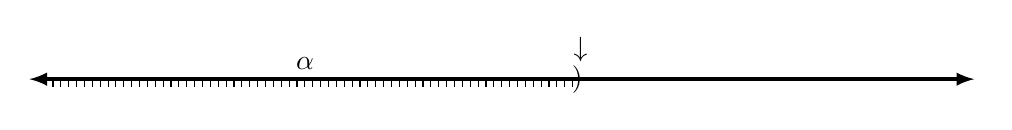
\begin{tikzpicture}
        \draw[latex-latex, very thick] (-6, 0) -- (6,0) node[anchor=south] {$\QQ$};
        \foreach \i in {-5.7,-5.6,...,0.9}{ 
        \draw[] (\i,0) -- (\i,-0.1);
        }
        \draw[] (1,0.1) node[anchor=south] {$\downarrow$};
        \draw[] (0.96,0) node[] {$)$};
        \draw[] (-2.5, 0) node[anchor=south] {$\alpha$};
    \end{tikzpicture}
    \caption{Visualization of a cut $\alpha$. The real number being described of this cut can be thought of as the number at the right boundary (the arrow).}
    \label{fig2} 
\end{figure}

\begin{nblank}{Step 2: $\RR$ is an ordered set}
    We define $\alpha < \beta$ to mean $\alpha \subsetneq \beta$. We show that this makes $\RR$ into an ordered set. First checking transitivity, we have that if $\alpha < \beta$ and $\beta < \gamma$ then $\alpha < \gamma$ by the fact that set inclusion is transitive. Furthermore, at most one of $\alpha < \beta$, $\alpha = \beta$, and $\beta < \alpha$ hold; to see this is the case, suppose the first two fail. Then, $\alpha \nsubseteq \beta$. Hence, $\exists p \in \alpha$ with $p \notin \beta$. If $q \in \beta$, $q < p$  and hence $q \in \alpha$ by (II), so $\beta \subset \alpha$, and since $\beta \neq \alpha$ it follows that $\beta \subsetneq \alpha$. 
\end{nblank}

\begin{nblank}{Step 3: $\RR$ has the LUB property}
    We show that $\RR$ has the LUB property. To see this is the case, let $A \subset \RR$ with $A \neq \emptyset$, and suppose that there exists $\beta \in \RR$ that is an upper bound for $A$. We will now define $\gamma = \bigcup_{\alpha \in A}\alpha$ and prove that $\gamma \in \RR$ and $\gamma = \sup A$ (hence $A$ has a supremum and $\RR$ has the LUB property).

    Since $A \neq \emptyset$, $\exists \alpha_0 \in A$, and since $\alpha_0 \neq \emptyset$ (as it is a cut) and $\alpha \subset \gamma$, it follows that $\gamma \neq \emptyset$. Next, we have that $\gamma \subset \beta$, since $\alpha \subset \beta$ for every $\alpha \in A$, and hence $\gamma \neq \QQ$, that is, $\gamma \subsetneq \QQ$. Hence $\gamma$ satisfies property (I) of a cut. 

    Take $p \in \gamma$. Then $p \in \alpha_1$ for some $\alpha_1 \in A$. If $q < p$, then $q \in \alpha$ (as $\alpha$ is a cut) so $q \in \gamma$, satisfying property (II).

    Next, choose $r \in \alpha_1$ such that $r > p$, then $r \in \gamma$ (as $\alpha_1 \subset \gamma$) and hence $\gamma$ satisfies property (III). Hence $\gamma$ is a cut, and $\gamma \in \RR$.

    Finally, we show that $\gamma = \sup A$. Clearly, $\alpha \leq \gamma$ for all $\alpha \in A$, as $\gamma = \bigcup_{\alpha \in A}\alpha$, so $\gamma$ is an upper boun dof $A$. To show that it is the least upper bound, let $\delta < \gamma$ be a cut. Then, $\exists s \in \gamma$ such that $s \notin \delta$. Therefore, $\exists \alpha_2 \in A$ such that $s \in \alpha_2$; hence $\delta < \alpha_2$, so $\delta$ is not an upper bound for $A$, giving the desired result. 
\end{nblank}

\begin{nblank}{Step 4: Addition on $\RR$}
    \begin{ndef}{Addition}
        If $\alpha, \beta \in \RR$, we define $\alpha + \beta = \set{s + t: s \in \alpha, t \in \beta}$. Showing that this is a cut is left as an exercise.
    \end{ndef}
    \begin{ndef}{Zero}
        $0^* = \set{s \in \QQ}$. Showing that this is a cut is left as an exercise.
    \end{ndef}

    We leave it as an exercise to show that the addition axioms (A1)-(A5) of a field are satisfied under this definition of addition on $\RR$, with the 0 element as $0^*$ defined above.
\end{nblank}

\begin{nblank}{Step 5: $\RR$ satisfies the Ordered Field Property (i)}
    We verify that if $\alpha, \beta, \gamma \in \RR$ and $\beta < \gamma$, then $\alpha + \beta < \alpha + \gamma$. 

    For every $s \in \alpha, t \in \beta$, we have that $t \in \gamma$ as $\beta$ is a subset of $\gamma$ by the definition of order on $\RR$. Hence, $s + t \in \alpha + \beta$ implies $s + t \in \alpha + \gamma$. Therefore, $\alpha + \beta \subseteq \alpha + \gamma$ and hence $\alpha + \beta \leq \alpha + \gamma$. 

    We are then left to check that $\alpha + \beta \neq \alpha + \gamma$. To see that this is the case, if $\alpha + \beta = \alpha + \gamma$, then $\beta = \alpha + \beta - \alpha = \alpha + \gamma - \alpha = \gamma$ by the field axioms for addition. Therefore we obtain that $\beta = \gamma$, contradicting that $\beta < \gamma$. Hence the claim is proven.

    As a remark, note that $0^* < \alpha \iff -\alpha < 0^*$.
\end{nblank}
\noindent Next we will define multiplication on $\RR$. A first attempt would be $\alpha \cdot \beta = \set{s \cdot t: s\in \alpha, t \in \beta}$. However, this doesn't work because we would not retain negative numbers. 
\begin{nblank}{Step 6: Positive Multiplication on $\RR$}
    \begin{ndef}{Positive Reals}
        We define $\RR^+ = \set{\alpha \in \RR: \alpha > 0^*}$
    \end{ndef}
    \begin{ndef}{Multiplication of Positive Reals}
        If $\alpha, \beta \in \RR^+$, we define $\alpha \cdot \beta = \set{r \cdot s: r \in \alpha, r> 0, s \in \beta, s > 0} \cup \set{t \in \QQ, t \leq 0}$. Equivalently, $\alpha \cdot \beta = \set{p \in \QQ:  \leq r \cdot s: r \in \alpha, r > 0, s \in \beta, s > 0}$. We leave it as an exercise to show that $\alpha \cdot \beta \in \RR$, and moreover, $\alpha \cdot \beta \in \RR^+$. Showing this second fact proves ordered field property (ii).
    \end{ndef}
    \begin{ndef}{One}
        $1^* = \set{r \in \QQ: r < 1}$. We again leave showing $1^* \in \RR^+$ as an exercise. 
    \end{ndef}
\end{nblank}

\begin{nblank}{Step 7: Multiplication on all of $\RR$}
    \begin{ndef}{Multiplication by zero}
        $\alpha \cdot 0^* = 0^* = 0^* \cdot \alpha$
    \end{ndef}
    \begin{ndef}{Multiplication}
        We define general multiplication as below, where the $\cdot$ on the RHS represents the multiplication of positive reals as outlined in Step 5. 
        \begin{align*}
            \alpha \cdot \beta = 
            \begin{cases}
            (-\alpha)\cdot(-\beta) & \text{if $\alpha < 0^*$ and $\beta < 0^*$}
            \\ -\left((-\alpha)\cdot\beta\right) & \text{if $\alpha < 0^*$ and $\beta > 0^*$}
            \\ -\left(\alpha \cdot (-\beta)\right) & \text{if $\alpha > 0^*$ and $\beta < 0^*$}
            \end{cases}
        \end{align*}
    \end{ndef}
    We leave it as an exercise to show that the multiplicative axioms (M1)-(M5), as well as the distributive law (D) of a field are satisfied under this definition of multiplication on $\RR$. 
\end{nblank}
\noindent Up until this point, we have shown $\RR$ is an ordered field with the LUB property; we last check that it contains $\QQ$ as a subfield. Note that we do have to be a bit careful with what we mean here; $\RR$ does not literally contain $\QQ$; $\RR$ is indeed a set of proper subsets of $\QQ$. What we really mean is to associate every element of $\QQ$ to an element of $\RR$ such that the field structure is preserved. 
\begin{nblank}{Step 8: $\RR$ contains $\QQ$ as a subfield}
    For each $r \in \QQ$, associate the cut $r^* = \set{p \in \QQ, p < r^*}$. We then leave as an easy exercise to verify that $r^* < s^* \iff r < s$, $r^* + s^* = r + s$, and $r^*\cdot s^* = r\cdot s$. This concludes the construction of the reals. \qed
\end{nblank}
\noindent Note that later on in the course, we will construct the real numbers in a different fashion; by considering Cauchy sequences modulo an equivalence relation. Also note that from here on out, it will suffice to have the standard/traditional picture of a "real number" in mind (i.e. infinite decimal expansions) and we will not have to really think about the real numbers as cuts; this was just necessary for the formal construction.

\subsection{The Complex Field}

\subsection{The Cauchy-Shwartz Inequality}

\subsection{Euclidean Space}


